\documentclass{beamer}

% Theme and Color Scheme
\usetheme{Boadilla}
\usecolortheme{seahorse}
\setbeamersize{text margin left=0.5cm, text margin right=0.5cm}
\setbeamertemplate{footline}{} % Remove footer
\date{}

% Required Packages
\usepackage{graphicx} % For including images
\usepackage{amsmath}  % For advanced math environments
\usepackage{amssymb}
\usepackage{booktabs} % For professional tables
\usepackage[numbers,sort&compress]{natbib} % For citations
\usepackage{qrcode} % For QR codes

% Title Page Information
\title[RMSTSS]{RMSTSS: A Comprehensive Software Suite for Power and Sample Size Calculation in Modern Clinical Trials}
\author{Arnab Aich}
\institute{Florida State University}
\date{\today}

\begin{document}

% ---------- Frame 1 ----------
\begin{frame}
  \titlepage
\end{frame}

% ---------- Frame 2 ----------
\section{Introduction \& Foundations}
\begin{frame}
\frametitle{The Fundamental Goal: Planning Better Clinical Trials}
Every clinical trial must answer two critical questions before it begins:

\begin{enumerate}
    \item \textbf{How many patients do we need?} (Sample Size Calculation)
    \item \textbf{What is our chance of detecting a real treatment effect?} (Statistical Power)
\end{enumerate}

\vspace{1em}

\begin{block}{Why is this relevant?}
\begin{itemize}
    \item \textbf{Ethical Responsibility:} Avoid exposing patients to ineffective treatments or running underpowered studies.
    \item \textbf{Resource Allocation:} Trials are expensive; proper planning ensures efficient use of time and funding.
    \item \textbf{Scientific Rigor:} A well-powered study is essential for valid and reliable inference.
\end{itemize}
\end{block}
\end{frame}

% ---------- Frame 3 ----------
\begin{frame}
\frametitle{The Standard Approach: Survival Models}
In many trials, the outcome is the \textbf{time until an event} occurs (e.g., recovery, disease progression, death).

\begin{block}{Key Notations}
\begin{itemize}
    \item $T$: true time-to-event; \quad $C$: censoring time
    \item Observed: $Y = \min(T, C)$; \quad $\delta = \mathbb{1}(T \le C)$
    \item \textbf{Survival Function} $S(t) = P(T > t)$
    \item \textbf{Hazard Function} $h(t) = \displaystyle \lim_{\Delta t \to 0} \frac{P(t \le T < t + \Delta t \mid T \ge t)}{\Delta t} = \frac{f(t)}{S(t)}$
\end{itemize}
\end{block}
\end{frame}

% ---------- Frame 4 ----------
\begin{frame}
\frametitle{The Proportional Hazards (PH) Assumption}
\begin{block}{What does this mean?}
The hazard in the treatment arm is a constant multiple of the hazard in control at all times \cite{cox1972}:
\[
h_1(t) = h_0(t) \cdot \theta.
\]
This implies a \textbf{constant relative risk reduction} throughout the study.
\end{block}

\begin{columns}
\begin{column}{0.5\textwidth}
    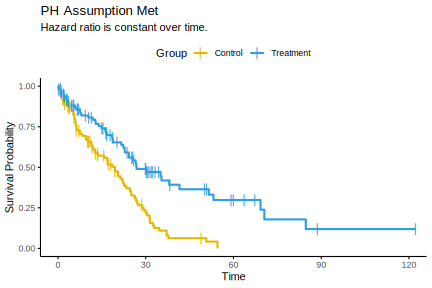
\includegraphics[width=\textwidth]{images/ph_assumption_met.png}
\end{column}
\begin{column}{0.5\textwidth}
    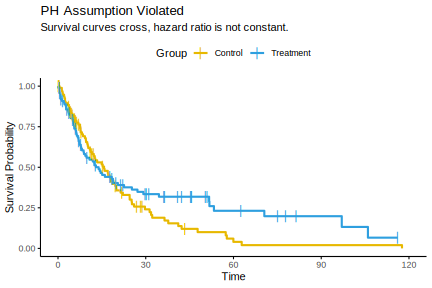
\includegraphics[width=\textwidth]{images/ph_assumption_violated.png}
\end{column}
\end{columns}
\end{frame}

% ---------- Frame 5 ----------
\begin{frame}
\frametitle{Problems with the Hazard Ratio}
\begin{enumerate}
    \item \textbf{PH is Often Violated}
    \begin{itemize}
        \item Modern therapies (e.g., immunotherapies) can show \textbf{delayed effects} or waning benefits.
        \item This leads to \textbf{crossing survival curves}, contradicting PH \cite{uno2014}.
    \end{itemize}
    \vspace{1em}
    \item \textbf{Limited Causal Interpretation}
    \begin{itemize}
        \item When PH fails, the Cox HR becomes a \textbf{time-averaged} summary and loses clear clinical meaning \cite{royston2013, uno2014}.
    \end{itemize}
\end{enumerate}
\end{frame}

% ---------- Frame 6 ----------
\begin{frame}
\frametitle{The Solution: Restricted Mean Survival Time (RMST)}
\begin{block}{Definition}
The RMST is the average event-free survival time up to a pre-specified horizon $L$:
\[
\mu(L) = E[\min(T, L)] = \int_0^L S(t)\, dt.
\]
\end{block}

\begin{block}{Interpretation \& Advantages}
\begin{itemize}
    \item \textbf{Directly Interpretable:} absolute time gained/lost (e.g., months).
    \item \textbf{No PH Required:} robust even when curves cross \cite{royston2013, uno2014}.
    \item \textbf{Clinically Meaningful:} patient-centered measure of benefit.
\end{itemize}
\end{block}
\end{frame}

% ---------- Frame 7 ----------
\begin{frame}
\frametitle{Causal Interpretation of the RMST Difference}
The treatment effect is the difference in RMST between the two arms.

\begin{block}{Causal Estimand}
\[
\Delta(L) = \mu_{\text{treatment}}(L) - \mu_{\text{control}}(L).
\]
\end{block}

\textbf{Interpretation:} $\Delta(L)$ is the \textbf{average gain in event-free time} attributable to treatment over $[0,L]$ \cite{uno2014}.
\end{frame}

% ---------- Frame 8 ----------
\begin{frame}
\frametitle{Causal Interpretation of RMST (PH Met vs.\ Violated)}
\begin{columns}
\begin{column}{0.5\textwidth}
\begin{block}{PH Met Case}
RMST reflects a clear average survival benefit.
\end{block}
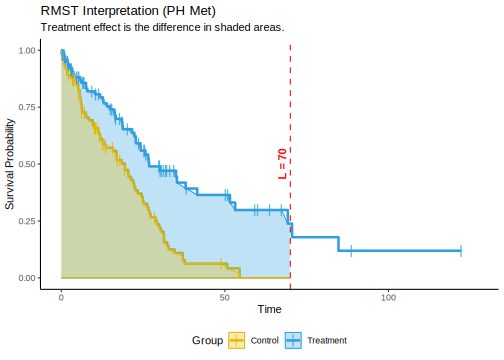
\includegraphics[width=\textwidth, height = 0.8\textwidth]{images/rmst_causal_plot_ph_met.png}
\end{column}
\begin{column}{0.5\textwidth}
\begin{block}{PH Violated Case}
RMST remains valid even with crossing curves.
\end{block}
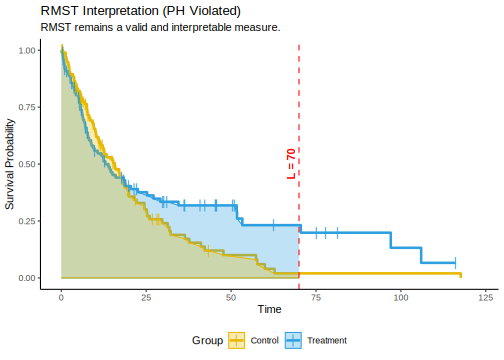
\includegraphics[width=\textwidth, height = 0.8\textwidth]{images/rmst_causal_plot_ph_violated.png}
\end{column}
\end{columns}

\small\textit{Treatment effect = difference in areas between curves \cite{royston2013}.}
\end{frame}

% ---------- Frame 9 ----------
\section{The RMSTSS Package: Models \& Methods}
\begin{frame}
\frametitle{Overview of Implemented Models}
\begin{figure}
    \centering
    \includegraphics[width=\linewidth]{images/app-models.png}
\end{figure}
\end{frame}

% ---------- Frame 10 ----------
\begin{frame}
\frametitle{Notation for Estimation}
For subject $i=1,\dots,n$:
\begin{itemize}
  \item $T_i$: event time; $C_i$: censoring time
  \item $Y_i = \min(T_i, C_i)$; \; $\delta_i = \mathbb{1}(T_i \le C_i)$
  \item $A_i \in \{0,1\}$: treatment (1 = treatment, 0 = control) \textit{(same as ``arm'' variable)}
  \item $Z_i$: baseline covariates; \; $S_i$: stratum (for multi-center trials)
\end{itemize}
\[
\mu(L) = E[\min(T,L)] = \int_0^L S(t)\,dt.
\]
\end{frame}

% ---------- Frame 11 ----------
\begin{frame}
\frametitle{Non-Stratified Model: Linear IPCW (after \cite{tian2014})}
\begin{block}{Model}
\[
E[\min(T_i,L) \mid A_i, Z_i] = \beta_0 + \beta_A A_i + \beta_Z^\top Z_i.
\]
\end{block}
\begin{block}{Challenge}
Direct regression on $Y_i$ fails under censoring; we use IPCW.
\end{block}
\begin{block}{Estimand}
$\beta_A$: adjusted RMST difference at horizon $L$.
\end{block}
\end{frame}

% ---------- Frame 12 ----------
\begin{frame}
\frametitle{Estimation with IPCW}
\begin{block}{Censoring Distribution}
Let $G(t) = P(C_i > t)$; estimate $\widehat{G}(t)$ by Kaplan--Meier (or Cox if covariate-dependent).
\end{block}
\begin{block}{Weights}
\[
w_i = \frac{\delta_i}{\widehat{G}(Y_i)}.
\]
\end{block}
\begin{block}{Weighted Least Squares}
\[
\widehat{\beta} = \arg\min_\beta \sum_{i=1}^n w_i \Big\{ Y_i - (\beta_0 + \beta_A A_i + \beta_Z^\top Z_i)\Big\}^2.
\]
\end{block}
\end{frame}

% ---------- Frame 13 ----------
\begin{frame}
\frametitle{Pseudo-Observations for RMST (after \cite{andersen2010})}
\begin{block}{Idea}
Replace censored outcomes by \textbf{pseudo-observations}.
\end{block}
\begin{block}{Definition}
Let $\widehat{\mu}(L)$ be RMST from the full sample and $\widehat{\mu}^{(-i)}(L)$ the leave-one-out version. Then
\[
\text{pseudo}_i(L) = n \cdot \widehat{\mu}(L) - (n-1)\cdot \widehat{\mu}^{(-i)}(L).
\]
\end{block}
\begin{block}{Key Property}
$E[\text{pseudo}_i(L)] = E[\min(T_i,L)]$.
\end{block}
\end{frame}

% ---------- Frame 14 ----------
\begin{frame}
\frametitle{Non-Stratified Model: Semiparametric GAM}
\begin{block}{Model}
\[
E[\text{pseudo}_i(L)] = \beta_0 + \beta_A A_i + \sum_{k=1}^{q} f_k(Z_{ik}),
\]
where $f_k(\cdot)$ are smooth spline functions \cite{hastie1990}.
\end{block}
\begin{block}{Estimand}
$\beta_A$: adjusted RMST difference allowing non-linear covariate effects.
\end{block}
\end{frame}

% ---------- Frame 15 ----------
\begin{frame}
\frametitle{Dependent Censoring (after \cite{wang2018})}
\begin{block}{Problem}
If censoring depends on covariates, a single $G(t)$ is biased.
\end{block}
\begin{block}{Cause-Specific Censoring Hazards}
For $K$ censoring causes with hazards $\lambda_{Ck}(t \mid Z_i)$ and cumulative hazards $\Lambda_{Ck}(t \mid Z_i)$:
\[
\widehat{G}(t \mid Z_i) = \exp\!\left\{-\sum_{k=1}^{K} \widehat{\Lambda}_{Ck}(t \mid Z_i)\right\}.
\]
Use $\widehat{G}(t \mid Z_i)$ in the IPCW weights \cite{robins1992}.
\end{block}
\end{frame}

% ---------- Frame 16 ----------
\begin{frame}
\frametitle{Stratified Models for Multi-Center Trials}
\begin{block}{Use Case}
Trials with many centers/strata where baseline RMST varies by stratum.
\end{block}
\begin{block}{Two Structures}
\begin{itemize}
    \item \textbf{Additive:} constant treatment benefit across strata.
    \item \textbf{Multiplicative:} proportional treatment benefit across strata.
\end{itemize}
\end{block}
\end{frame}

% ---------- Frame 17 ----------
\begin{frame}
\frametitle{Stratified Model 1: Additive (after \cite{zhang2024})}
\begin{block}{Model}
\[
E[\min(T_i,L) \mid A_i, Z_i, S_i=j] = \alpha_j + \beta_A A_i + \beta_Z^\top Z_i.
\]
\end{block}
\begin{block}{Estimand}
$\beta_A$: \textbf{common additive} RMST difference across strata.
\end{block}
\end{frame}

% ---------- Frame 18 ----------
\begin{frame}
\frametitle{Stratified Model 2: Multiplicative (after \cite{wang2019})}
\begin{block}{Model (log-mean form)}
\[
\log E[\min(T_i,L) \mid A_i, Z_i, S_i=j] = \alpha_j + \beta_A A_i + \beta_Z^\top Z_i,
\]
equivalently,
\[
E[\min(T_i,L) \mid A_i, Z_i, S_i=j] = \exp(\alpha_j)\exp(\beta_A A_i)\exp(\beta_Z^\top Z_i).
\]
\end{block}
\begin{block}{Estimand}
$\exp(\beta_A)$: \textbf{RMST ratio} (treatment vs.\ control), common across strata.
\end{block}
\end{frame}

% ---------- Frame 19 ----------
\section{Power \& Sample Size with RMSTSS}
\begin{frame}
\frametitle{Core Computational Approaches}
\begin{block}{Analytical (variance-based)}
\[
\text{Power} = 
\Phi\!\left( \frac{|\widehat{\beta}_A|}{\widehat{\sigma}_{\beta_A}/\sqrt{n}} - z_{1-\alpha/2}\right),
\]
leveraging large-sample variance of $\widehat{\beta}_A$ \cite{royston2013}.
\end{block}

\begin{block}{Bootstrap (pilot resampling)}
\[
\text{Power} = \frac{\#\{\text{replicates with $p<\alpha$}\}}{B},
\]
robust to complex censoring and model misspecification.
\end{block}
\end{frame}

% ---------- Frame 20 ----------
\begin{frame}
\frametitle{Package Functionality \& Naming Convention}
Functions follow a consistent pattern:
\[
\texttt{model.goal.method()}.
\]

\begin{itemize}
  \item \textbf{Model:} \texttt{linear}, \texttt{GAM}, \texttt{DC}, \texttt{additive}, \texttt{MS}
  \item \textbf{Goal:} \texttt{power} (estimate power) or \texttt{ss} (sample size for target power)
  \item \textbf{Method:} \texttt{analytical} or \texttt{boot}
\end{itemize}

\textbf{Example:} \texttt{MS.ss.boot()} $\Rightarrow$ sample size for the Multiplicative Stratified model using bootstrap.
\end{frame}

% ---------- Frame 21 ----------
\begin{frame}
\frametitle{RMSTSS Function Reference (by goal)}
\small
\begin{tabular}{@{}lll@{}}
\toprule
\textbf{Design Goal} & \textbf{Model} & \textbf{Functions} \\
\midrule
Power & Non-stratified linear & \texttt{linear.power.analytical()}, \texttt{linear.power.boot()} \\
Power & Non-stratified GAM & \texttt{GAM.power.analytical()}, \texttt{GAM.power.boot()} \\
Power & Dependent censoring & \texttt{DC.power.analytical()}, \texttt{DC.power.boot()} \\
Power & Stratified additive & \texttt{additive.power.analytical()}, \texttt{additive.power.boot()} \\
Power & Stratified multiplicative & \texttt{MS.power.analytical()}, \texttt{MS.power.boot()} \\
\midrule
Sample size & Non-stratified linear & \texttt{linear.ss.analytical()}, \texttt{linear.ss.boot()} \\
Sample size & Non-stratified GAM & \texttt{GAM.ss.analytical()}, \texttt{GAM.ss.boot()} \\
Sample size & Dependent censoring & \texttt{DC.ss.analytical()}, \texttt{DC.ss.boot()} \\
Sample size & Stratified additive & \texttt{additive.ss.analytical()}, \texttt{additive.ss.boot()} \\
Sample size & Stratified multiplicative & \texttt{MS.ss.analytical()}, \texttt{MS.ss.boot()} \\
\bottomrule
\end{tabular}

\vspace{0.6em}
\footnotesize Core args: \texttt{pilot\_data}, \texttt{time\_var}, \texttt{status\_var}, \texttt{arm\_var}, \texttt{L}; stratified adds \texttt{strata\_var}; bootstrap adds \texttt{n\_boot}, \texttt{seed}.
\end{frame}

% ---------- Frame 22 ----------
\begin{frame}[fragile]
\frametitle{Worked Example: Sample Size (Additive, Analytical)}
\scriptsize
\begin{verbatim}
library(survival)
library(RMSTSS)

# Prepare pilot data
colon_death <- colon[colon$etype == 2, ] %>% na.omit()
colon_death$arm <- ifelse(colon_death$rx == "Obs", 0, 1)
colon_death$strata <- factor(colon_death$extent)

# Analytical sample size
ss_results <- additive.ss.analytical(
  pilot_data   = colon_death,
  time_var     = "time",
  status_var   = "status",
  arm_var      = "arm",
  strata_var   = "strata",
  target_power = 0.80,
  L            = 1825
)

print(ss_results$results_data)
\end{verbatim}
\end{frame}

% ---------- Frame 23 ----------
\begin{frame}[fragile]
\frametitle{Worked Example: Sample Size (Additive, Bootstrap)}
\scriptsize
\begin{verbatim}
# Bootstrap sample size
ss_boot <- additive.ss.boot(
  pilot_data   = colon_death,
  time_var     = "time",
  status_var   = "status",
  arm_var      = "arm",
  strata_var   = "strata",
  target_power = 0.80,
  L            = 1825,
  n_boot       = 500,   # bootstrap replicates
  seed         = 2025
)

print(ss_boot$results_data)
\end{verbatim}

\small The bootstrap approach simulates variability from the pilot data, offering robustness under complex censoring patterns.
\end{frame}

% ---------- Frame 24 ----------
\section{Software \& Application}
\begin{frame}
\frametitle{The \texttt{RMSTSS} Shiny Application}
\begin{block}{Key Features}
\begin{itemize}
  \item Upload pilot data in \texttt{.csv} format
  \item Map columns (time, status, treatment, strata) via dropdowns
  \item Select model (\texttt{linear}, \texttt{GAM}, \texttt{additive}, \texttt{MS}, \texttt{DC})
  \item Choose goal (\texttt{power} or \texttt{ss}) and method (\texttt{analytical} or \texttt{boot})
  \item Interactive outputs: survival curves, power curves
  \item Export analysis reports (pdf)
\end{itemize}
\end{block}
\end{frame}

% ---------- Frame 25 ----------
\begin{frame}
\frametitle{Application Interface (Analysis Panel)}
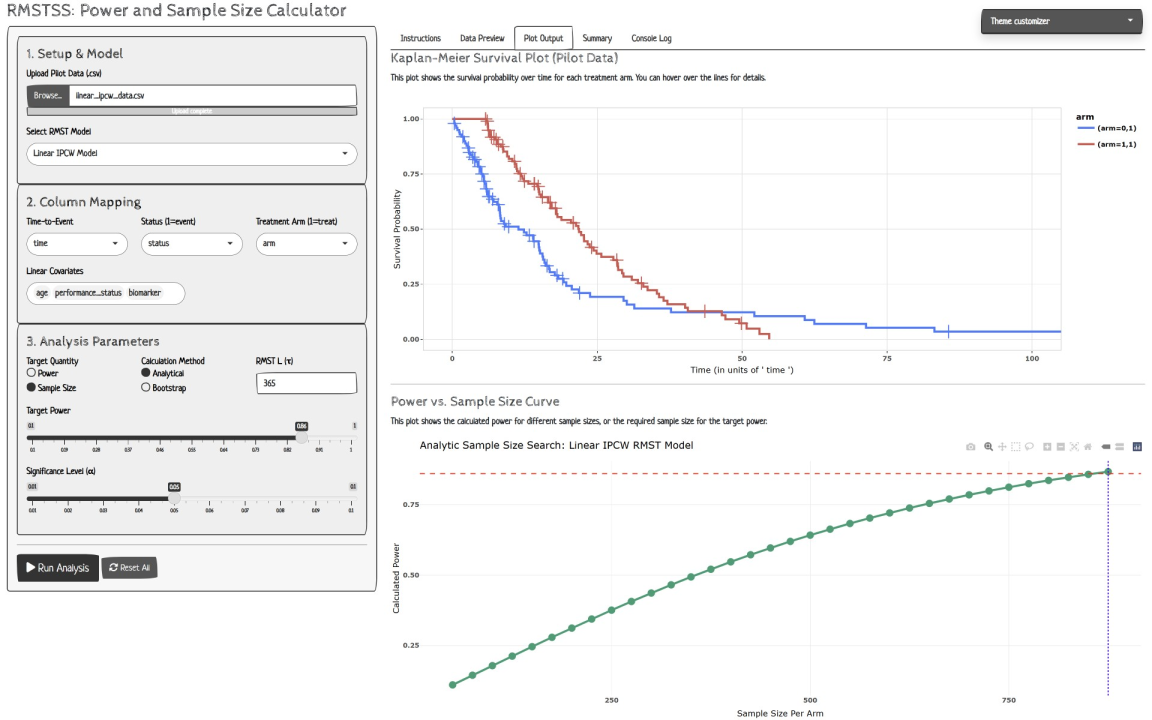
\includegraphics[width=\textwidth]{images/app-ss.png}
\end{frame}

% ---------- Frame 26 ----------
\begin{frame}
\frametitle{Application Interface (Full-Screen View)}
\includegraphics[width=\paperwidth,height=\paperheight,keepaspectratio]{images/app-interface-full.png}
\end{frame}

% ---------- Frame 27 ----------
\section{Conclusion}
\begin{frame}
\frametitle{Conclusion \& Future Aims}

\begin{block}{Conclusion}
\begin{itemize}
  \item \textbf{Statistically Rigorous:} Linear, GAM, dependent censoring, and stratified RMST models
  \item \textbf{Causally Interpretable:} RMST difference $\beta_A$ or RMST ratio $\exp(\beta_A)$
  \item \textbf{Practical:} Delivered as both an R package and a Shiny web application
\end{itemize}
\end{block}

\begin{block}{Future Aims}
\begin{itemize}
  \item Extend to \textbf{time-varying treatments} and adaptive trial designs
  \item Incorporate \textbf{Bayesian approaches} for RMST-based planning
  \item Modules for \textbf{multi-arm and platform trials}
  \item Improve app interactivity with \textbf{dynamic simulation dashboards}
\end{itemize}
\end{block}
\end{frame}

% ---------- Frame 28 ----------
\begin{frame}[allowframebreaks]
\frametitle{References}
\scriptsize
\bibliographystyle{plainnat}
\bibliography{references}
\end{frame}

% ---------- Frame 29 ----------
\begin{frame}
\frametitle{Access \& Acknowledgments}
\begin{columns}[T]
\begin{column}{0.5\textwidth}
\scriptsize
    \textbf{Acknowledgments}
 \begin{itemize}
        \item Grateful appreciation to Dr.\ Yuan Zhang (UTHSC) for mentorship
        \item Special thanks to Dr.\ Gregory Farage and Dr.\ Saunak Sen (UTHSC)
        \item Support from UTHSC BERD (Biostatistics, Epidemiology, and Research Design)
        \item Funded by NSF Grant No.\ 2220726
    \end{itemize}
\vfill
\begin{center}
\Huge{\textbf{Questions?}}
\end{center}
\end{column}
    \begin{column}{0.5\textwidth}
    \scriptsize
        \centering
        \textbf{Scan for Web App} \\
        \qrcode[height=3cm]{https://arnab96.shinyapps.io/uthsc-app/}
        \vspace{2em} \\
        \textbf{Scan for R Package} \\
        \qrcode[height=3cm]{https://github.com/arnab-aich/RMSTSS}
    \end{column}
\end{columns}
\end{frame}

\end{document}

